\documentclass[
	letterpaper, % Paper size, specify a4paper (A4) or letterpaper (US letter)
	10pt, % Default font size, specify 10pt, 11pt or 12pt
]{CSUniSchoolLabReport}

%----------------------------------------------------------------------------------------
%	REPORT INFORMATION
%----------------------------------------------------------------------------------------

\title{Final Project: Hangman\\ Computing Fundamentals\\ EECE2140} % Report title

\author{Michael \textsc{Brodskiy}\\ \small \href{mailto:Brodskiy.M@Northeastern.edu}{Brodskiy.M@Northeastern.edu}}

\date{April 28, 2023} % Date of the report

%----------------------------------------------------------------------------------------


\begin{document}

\maketitle % Insert the title, author and date using the information specified above

\begin{center}
	\begin{tabular}{l r}
		Instructor: & Professor \textsc{Fanaei} % Instructor/supervisor
	\end{tabular}
\end{center}

\newpage

\section{Introduction}

The purpose of the final project in this course is to unify concepts covered throughout the entirety of the course; as such, this final project recreates the popular hangman game. There are two modes, single and multi player. When single player is selected, a word is selected at random (using the \texttt{random} module) from a word bank. The player then has two options: guessing a letter or guessing the phrase, both of which work as one would expect. Every time a letter is guessed, it is added to the list of guessed letters, which stop the player from guessing the same letter twice. The guesser has 5 attempts to guess correctly until they are ``hung''. The difference between single and multi player is that, with multiplayer, a custom phrase may be entered. Once a game ends, the user is prompted whether they want to play again, and the process is restarted.\\

On the technical side of things, two classes are implemented in the code: \texttt{hangman} and \texttt{game}. The \texttt{game} class inherits from the \texttt{hangman} class, which is essentially just a class to display the text-based hangman figure. The \texttt{game} class contains several functions, each of which is used to implement a certain aspect of the game, such as \texttt{end()}, which checks whether the game should end, \texttt{enter\_phrase}, which handles custom phrase input, and \texttt{generate\_secret}, which converts an entered phrase to underscores and spaces. Together with the code to create a \texttt{game} object, the game may be easily implemented and played.

\section{Components}

First and foremost, there is the \texttt{hangman} class, which is essentially just used to create a hangman figure. Within it, there is an \texttt{\_\_init\_\_()} function, which is not very important, and an \texttt{\_\_str\_\_()} function, which prints the figure.

The \texttt{game} class inherits the hangman class, but has much more functionality in terms of running the actual game. The functions it contains are as follows:

\begin{itemize}

  \item \texttt{\_\_init\_\_()} — Initializes the superclass, and creates \texttt{mode}, \texttt{limbs\_lost}, \texttt{totalguesses}, and \texttt{guessedLetters} class attributes.

  \item \texttt{mode} getters and setters — Used to verify that \texttt{mode} is always either 0 or 1

  \item \texttt{enter\_word()} — Executes the \texttt{generate\_secret()} function, and stores the word in the \texttt{word} class attribute

  \item \texttt{guess\_part()} — Used to guess a letter

    \begin{itemize}

      \item If more than a single letter is entered, causes exits function

      \item Adds the guessed letter to the \texttt{guessedLetters} list, if not there already; if it is already there, exits the function

      \item Checks for the index of the guess; catches a ValueError by setting \texttt{index} to 1 instead; if the index is not -1, each instance of a letter is replaced, and the \texttt{totalguesses} attribute is increased by one; if the index is -1 (not found), the player loses a limb (\texttt{limbs\_lost} is increased by 1), and \texttt{totalguesses} is increased

    \end{itemize}

  \item \texttt{guess\_phrase()} — Used to check whether the user has entered the correct phrase; if yes, the game ends and user wins; if not, the user loses a limb and the game continues.

  \item \texttt{generate\_word()} — Uses the \texttt{random} module to randomly select a word from a word bank (for single player mode)

  \item \texttt{generate\_secret()} — Converts an entered word to underscores for the letters and keeps spaces as spaces

  \item \texttt{end()} — Also implements exception handling to determine whether the game has ended (all limbs lost or all letters guessed)

  \item \texttt{menu()} — Used to print a menu to ask whether the user would like to enter a letter or phrase

  \item \texttt{play()} — Implements all of the above functionality, in addition to the \texttt{\_\_str\_\_()} function to run the actual game

  \item \texttt{\_\_str\_\_()} — Uses the string function from \texttt{hangman}, in addition to class attributes, to print a tui game window

\end{itemize}

The main code simply contains some code to request a mode selection by the user, create a \texttt{game} object, and, upon game end, asks whether the user would like to play again (using a \texttt{while} loop)

\section{Running the Code}

Given that this project is contained within a single file, the only necessity is to have the \texttt{random} module installed; the project may be run with the following command:

\begin{center}
  \texttt{>\_ python3 hangman.py}
\end{center}

\section{External Libraries}

The only external library used was the \texttt{random} module

\section{Conclusion}

The implementation of this program, most importantly, solidified two concepts for me: the idea of object-oriented programming in python, and the use of exception handling. It took me some time to figure out why simply using \texttt{<something>.index(<text>) == -1} did not work, and how to fix it. Additionally, using protected classes and inheritance allowed me to get a better feel for abstraction, and the fabrication of an input-based \texttt{\_\_str\_\_()} function allowed for a greater understanding of polymorphism.

\section{Appendix}

\lstinputlisting[
    caption=Full Program Code, % Caption above the listing
	label=lst:L1, % Label for referencing this listing
	language=python, % Use python functions/syntax highlighting
	frame=single, % Frame around the code listing
	showstringspaces=false, % Don't put marks in string spaces
	numbers=left, % Line numbers on left
	numberstyle=\tiny, % Line numbers styling
    backgroundcolor=\color{black!5}, % Set background color
    keywordstyle=\color{magenta!80}, % Set keyword color
    commentstyle=\color{blue!80}, % Set comment color
    stringstyle=\color{green!80}, % Set string color
    breaklines=true
  ]{project/hangman.py}

  \begin{figure}[H]
    \centering
    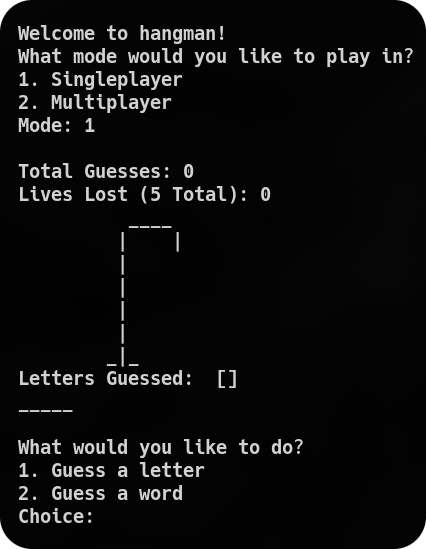
\includegraphics[width=.6\textwidth]{Figures/singleplayer.png}
    \caption{Launching a Single Player Game}
    \label{fig:1}
  \end{figure}

  \begin{figure}[H]
    \centering
    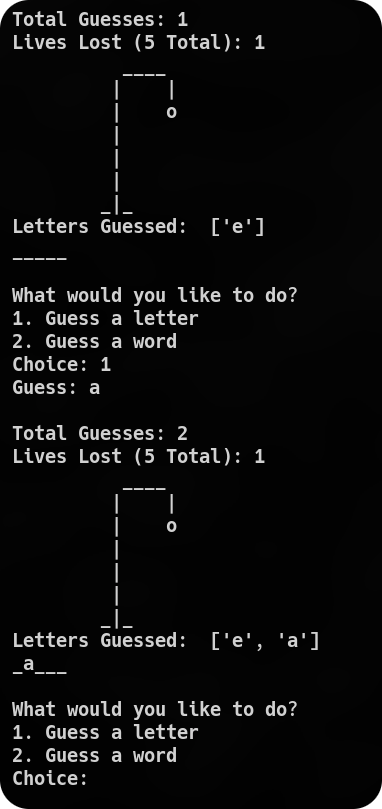
\includegraphics[width=.6\textwidth]{Figures/onerightonewrong.png}
    \caption{One Right, One Wrong Guess}
    \label{fig:2}
  \end{figure}

  \begin{figure}[H]
    \centering
    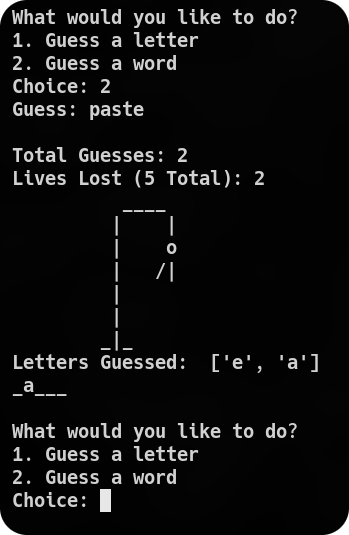
\includegraphics[width=.6\textwidth]{Figures/guessphrase.png}
    \caption{Guessing a Phrase}
    \label{fig:3}
  \end{figure}

  \begin{figure}[H]
    \centering
    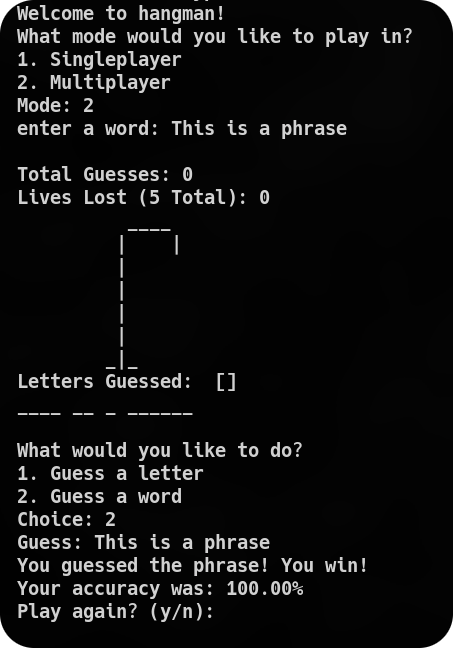
\includegraphics[width=.6\textwidth]{Figures/multiplayer.png}
    \caption{Multiplayer Game}
    \label{fig:4}
  \end{figure}

\end{document}
